% Battery cell schematic and the five database properties. Build: tectonic battery_cell.tex
\documentclass[tikz,border=4pt]{standalone}
\usepackage[T1]{fontenc}
\usepackage{tgheros}
\renewcommand{\familydefault}{\sfdefault}
\usepackage{amsmath}
\usepackage{sansmath}\sansmath
\usetikzlibrary{arrows.meta,positioning,calc,decorations.pathmorphing,patterns}

\definecolor{al}{RGB}{176,183,192}
\definecolor{cu}{RGB}{200,128,84}
\definecolor{cath}{RGB}{74,120,168}
\definecolor{cathlt}{RGB}{214,226,239}
\definecolor{anod}{RGB}{88,88,96}
\definecolor{anodlt}{RGB}{226,226,230}
\definecolor{elec}{RGB}{236,244,230}
\definecolor{sep}{RGB}{252,250,240}
\definecolor{li}{RGB}{214,69,80}
\definecolor{pcap}{RGB}{47,93,138}
\definecolor{pvolt}{RGB}{201,123,74}
\definecolor{pcond}{RGB}{88,160,104}
\definecolor{pce}{RGB}{140,110,180}
\definecolor{pen}{RGB}{181,80,90}
\definecolor{note}{RGB}{125,125,125}

\tikzset{
  lbl/.style={font=\footnotesize,align=center},
  prop/.style={draw=#1,line width=0.8pt,rounded corners=2pt,fill=#1!8,font=\scriptsize,align=left,inner sep=3pt,text width=3.35cm},
  ion/.style={circle,fill=li,inner sep=0pt,minimum size=4.2pt},
  arr/.style={-{Stealth[length=4pt]},line width=0.7pt},
}

\begin{document}
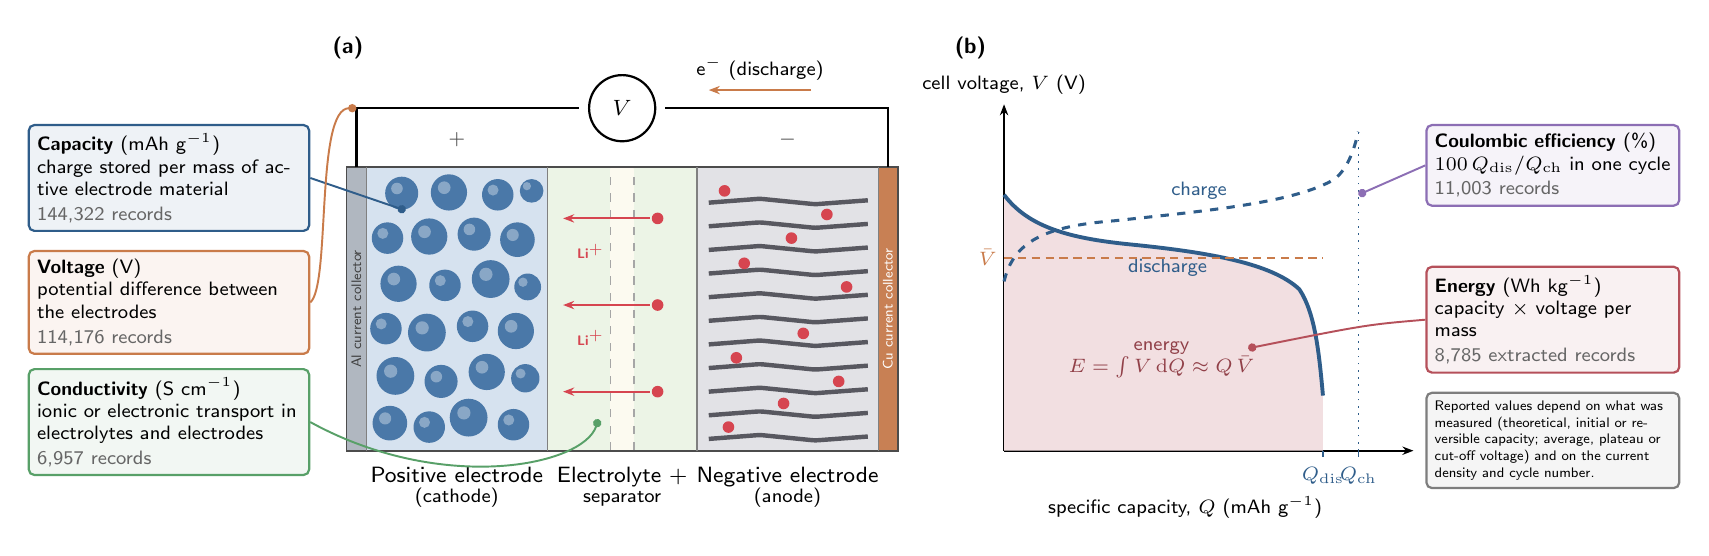
\begin{tikzpicture}[x=1cm,y=1cm]

% ===================================================== (a) cell cross-section
\def\H{3.6}
% current collectors
\fill[al] (0,0) rectangle (0.25,\H); \draw[black!60] (0,0) rectangle (0.25,\H);
\fill[cu] (6.75,0) rectangle (7.0,\H); \draw[black!60] (6.75,0) rectangle (7.0,\H);
% cathode (positive electrode)
\fill[cathlt] (0.25,0) rectangle (2.55,\H);
\foreach \x/\y/\r in {0.55/0.35/0.22,1.05/0.30/0.20,1.55/0.42/0.24,2.12/0.33/0.2,
                      0.62/0.95/0.24,1.20/0.88/0.21,1.78/1.00/0.23,2.27/0.92/0.18,
                      0.50/1.55/0.2,1.02/1.50/0.24,1.60/1.58/0.2,2.15/1.52/0.23,
                      0.66/2.12/0.23,1.25/2.10/0.2,1.83/2.18/0.24,2.30/2.08/0.17,
                      0.52/2.70/0.2,1.05/2.72/0.23,1.62/2.75/0.21,2.17/2.68/0.22,
                      0.70/3.27/0.21,1.30/3.28/0.23,1.92/3.25/0.2,2.35/3.30/0.15}
  {\fill[cath] (\x,\y) circle (\r); \fill[white,opacity=0.35] (\x-0.06,\y+0.06) circle (\r*0.35);}
% separator / electrolyte
\fill[elec] (2.55,0) rectangle (4.45,\H);
\fill[sep] (3.35,0) rectangle (3.65,\H);
\draw[black!35,dashed] (3.35,0) -- (3.35,\H) (3.65,0) -- (3.65,\H);
% anode (negative electrode): stacked graphite sheets
\fill[anodlt] (4.45,0) rectangle (6.75,\H);
\foreach \yy in {0.15,0.45,...,3.45}
  {\draw[anod,line width=1.6pt,rounded corners=1pt] (4.6,\yy) -- (5.25,\yy+0.05) -- (5.95,\yy-0.02) -- (6.62,\yy+0.03);}
% lithium ions (in anode between sheets, in electrolyte travelling)
\foreach \x/\y in {4.85/0.30,5.55/0.60,6.25/0.88,4.95/1.18,5.80/1.49,6.35/2.08,5.05/2.38,5.65/2.70,6.10/3.00,4.80/3.30}
  {\node[ion] at (\x,\y) {};}
\foreach \y in {0.75,1.85,2.95}
  {\node[ion] (i\y) at (3.95,\y) {}; \draw[arr,li] (3.85,\y) -- (2.75,\y);}
\node[font=\tiny\bfseries,text=li] at (3.10,1.43) {Li$^{+}$};
\node[font=\tiny\bfseries,text=li] at (3.10,2.53) {Li$^{+}$};
\draw[black!70,line width=0.6pt] (0,0) rectangle (7,\H);
\foreach \x in {0.25,2.55,4.45,6.75} \draw[black!50] (\x,0) -- (\x,\H);
% labels under the cell
\node[rotate=90,font=\tiny,text=black!75] at (0.125,\H/2) {Al current collector};
\node[lbl,anchor=north] at (1.40,-0.08) {Positive electrode\\[-2pt]{\scriptsize (cathode)}};
\node[lbl,anchor=north] at (3.50,-0.08) {Electrolyte +\\[-2pt]{\scriptsize separator}};
\node[lbl,anchor=north] at (5.60,-0.08) {Negative electrode\\[-2pt]{\scriptsize (anode)}};
\node[rotate=90,font=\tiny,text=white] at (6.875,\H/2) {Cu current collector};
% external circuit
\draw[line width=0.8pt] (0.125,\H) -- (0.125,\H+0.75) -- (2.95,\H+0.75);
\draw[line width=0.8pt] (4.05,\H+0.75) -- (6.875,\H+0.75) -- (6.875,\H);
\draw[line width=0.8pt,fill=white] (3.5,\H+0.75) circle (0.42);
\node[font=\footnotesize\bfseries] at (3.5,\H+0.75) {$V$};
\draw[arr,pvolt] (5.9,\H+0.98) -- (4.6,\H+0.98) node[midway,above,font=\scriptsize,text=black] {e$^{-}$ (discharge)};
\node[font=\footnotesize\bfseries,anchor=south west] at (-0.3,\H+1.25) {(a)};
\node[font=\scriptsize,text=black!70] at (1.40,\H+0.35) {$+$};
\node[font=\scriptsize,text=black!70] at (5.60,\H+0.35) {$-$};

% property call-outs for (a)
\node[prop=pcap,anchor=north west] (pc) at (-4.05,\H+0.55)
  {\textbf{Capacity} (mAh g$^{-1}$)\\charge stored per mass of active electrode material\\[1pt]\textcolor{black!60}{144,322 records}};
\draw[pcap,line width=0.7pt,-{Circle[length=3pt]}] (pc.east) -- (0.75,\H-0.55);
\node[prop=pvolt,anchor=north west] (pv) at (-4.05,\H-1.05)
  {\textbf{Voltage} (V)\\potential difference between the electrodes\\[1pt]\textcolor{black!60}{114,176 records}};
\draw[pvolt,line width=0.7pt,-{Circle[length=3pt]}] (pv.east) .. controls (-0.2,\H-1.5) and (-0.4,\H+0.75) .. (0.125,\H+0.75);
\node[prop=pcond,anchor=north west] (pk) at (-4.05,\H-2.55)
  {\textbf{Conductivity} (S cm$^{-1}$)\\ionic or electronic transport in electrolytes and electrodes\\[1pt]\textcolor{black!60}{6,957 records}};
\draw[pcond,line width=0.7pt,-{Circle[length=3pt]}] (pk.east) .. controls (1.2,-0.55) and (3.0,-0.2) .. (3.2,0.4);

% ===================================================== (b) galvanostatic cycle
\begin{scope}[shift={(8.35,0)}]
\node[font=\footnotesize\bfseries,anchor=south west] at (-0.75,\H+1.25) {(b)};
\draw[arr,black] (0,0) -- (5.2,0) ;
\node[font=\scriptsize] at (2.3,-0.72) {specific capacity, $Q$ (mAh g$^{-1}$)};
\draw[arr,black] (0,0) -- (0,4.4) node[above,font=\scriptsize] {cell voltage, $V$ (V)};
% energy area under discharge curve
\fill[pen!18] (0,3.25) .. controls (0.3,2.85) and (0.8,2.7) .. (1.6,2.62)
      .. controls (2.6,2.52) and (3.4,2.38) .. (3.75,2.05) .. controls (3.95,1.75) and (4.0,1.25) .. (4.05,0.7)
      -- (4.05,0) -- (0,0) -- cycle;
% charge curve (dashed)
\draw[pcap,line width=1.1pt,dashed] (0,2.15) .. controls (0.12,2.65) and (0.5,2.85) .. (1.4,2.92)
      .. controls (2.6,3.05) and (3.7,3.15) .. (4.2,3.45) .. controls (4.38,3.6) and (4.45,3.85) .. (4.5,4.05);
% discharge curve
\draw[pcap,line width=1.4pt] (0,3.25) .. controls (0.3,2.85) and (0.8,2.7) .. (1.6,2.62)
      .. controls (2.6,2.52) and (3.4,2.38) .. (3.75,2.05) .. controls (3.95,1.75) and (4.0,1.25) .. (4.05,0.7);
\node[font=\scriptsize,text=pcap,anchor=west] at (2.0,3.30) {charge};
\node[font=\scriptsize,text=pcap,anchor=west] at (1.45,2.32) {discharge};
% average voltage
\draw[pvolt,line width=0.8pt,densely dashed] (0,2.45) -- (4.05,2.45);
\node[font=\scriptsize,text=pvolt,anchor=east,fill=white,inner sep=1pt] at (-0.05,2.45) {$\bar V$};
% capacities
\draw[pcap,line width=0.6pt] (4.05,0) -- (4.05,-0.08) node[below,font=\scriptsize] {$Q_\mathrm{dis}$};
\draw[pcap,line width=0.6pt,dotted] (4.5,0) -- (4.5,4.05);
\draw[pcap,line width=0.6pt] (4.5,0) -- (4.5,-0.08) node[below,font=\scriptsize] {$Q_\mathrm{ch}$};
% energy label
\node[font=\scriptsize,text=pen!80!black,align=center] at (2.0,1.15) {energy\\$E=\int V\,\mathrm{d}Q\approx Q\,\bar V$};

% call-outs for (b)
\node[prop=pce,anchor=north west,text width=3.0cm] (pe) at (5.35,\H+0.55)
  {\textbf{Coulombic efficiency} (\%)\\$100\,Q_\mathrm{dis}/Q_\mathrm{ch}$ in one cycle\\[1pt]\textcolor{black!60}{11,003 records}};
\draw[pce,line width=0.7pt,-{Circle[length=3pt]}] (pe.west) -- (4.5,3.25);
\node[prop=pen,anchor=north west,text width=3.0cm] (pn) at (5.35,\H-1.25)
  {\textbf{Energy} (Wh kg$^{-1}$)\\capacity $\times$ voltage per mass\\[1pt]\textcolor{black!60}{8,785 extracted records}};
\draw[pen,line width=0.7pt,-{Circle[length=3pt]}] (pn.west) .. controls (4.6,1.6) .. (3.1,1.3);
\node[prop=note,anchor=north west,text width=3.0cm,font=\tiny] at (5.35,\H-2.85)
  {Reported values depend on what was measured (theoretical, initial or reversible capacity; average, plateau or cut-off voltage) and on the current density and cycle number.};
\end{scope}
\end{tikzpicture}
\end{document}
